%---------------------------------------------------------------------
%
%                         Project Name:Njust LabReport 
%
%---------------------------------------------------------------------
%
%                 created by Qingyun Fang <fqy2017@gmail.com>
%
%                        Last-modified: 2017-6-12
%
%---------------------------------------------------------------------

\documentclass[a4paper,12pt]{report}
\usepackage{etex}
\usepackage{ctex}
%\usepackage{xeCJK}
\usepackage{times}
\usepackage{setspace}
\usepackage{fancyhdr}
\usepackage{graphicx}
\usepackage{wrapfig}
\usepackage{array}  
\usepackage{fontspec,xunicode,xltxtra}
\usepackage{titlesec}
\usepackage{titletoc}
\usepackage[titletoc]{appendix}
\usepackage[top=30mm,bottom=30mm,left=20mm,right=20mm]{geometry}
\usepackage{cite}
\usepackage{listings}
\usepackage{caption,subcaption}
\usepackage[framed,numbered,autolinebreaks,useliterate]{mcode} % 插入代码
\usepackage{xeboiboites}
\usepackage{amsmath,amssymb}
\usepackage{hyperref}

\RequirePackage{tkz-network}

\hypersetup{hidelinks}

\XeTeXlinebreaklocale "zh"
\XeTeXlinebreakskip = 0pt plus 1pt minus 0.1pt

%---------------------------------------------------------------------
%	页眉页脚设置
%---------------------------------------------------------------------
\fancypagestyle{plain}{
	\pagestyle{fancy}      %改变章节首页页眉
}

\pagestyle{fancy}
\lhead{\kaishu~宜通华盛~}
\rhead{\kaishu~通信项目组~}
\cfoot{\thepage}

%---------------------------------------------------------------------
%	章节标题设置
%---------------------------------------------------------------------
\titleformat{\chapter}{\centering\zihao{-1}\heiti}{仿真实验\chinese{chapter}}{1em}{}
\titlespacing{\chapter}{0pt}{*0}{*6}

%---------------------------------------------------------------------
%	摘要标题设置
%---------------------------------------------------------------------
\renewcommand{\abstractname}{\zihao{-3} 摘\quad 要}

%---------------------------------------------------------------------
%	参考文献设置
%---------------------------------------------------------------------
\renewcommand{\bibname}{\zihao{2}{\hspace{\fill}参\hspace{0.5em}考\hspace{0.5em}文\hspace{0.5em}献\hspace{\fill}}}

%---------------------------------------------------------------------
%	引用文献设置为上标
%---------------------------------------------------------------------
\makeatletter
\def\@cite#1#2{\textsuperscript{[{#1\if@tempswa , #2\fi}]}}
\makeatother

%---------------------------------------------------------------------
%	目录页设置
%---------------------------------------------------------------------
\titlecontents{chapter}[0em]{\songti\zihao{-4}}{\thecontentslabel\ }{}
{\hspace{.5em}\titlerule*[4pt]{$\cdot$}\contentspage}
\titlecontents{section}[2em]{\vspace{0.1\baselineskip}\songti\zihao{-4}}{\thecontentslabel\ }{}
{\hspace{.5em}\titlerule*[4pt]{$\cdot$}\contentspage}
\titlecontents{subsection}[4em]{\vspace{0.1\baselineskip}\songti\zihao{-4}}{\thecontentslabel\ }{}
{\hspace{.5em}\titlerule*[4pt]{$\cdot$}\contentspage}

%---------------------------------------------------------------------
%	公式设置
%---------------------------------------------------------------------
%%define the newthem environment
\newboxedtheorem[small box style={fill=blue!20,draw=black, 
    rounded corners},
    big box style={fill=blue!10,draw=orange,thick,rounded corners},
    headfont=\bfseries]%
    {proposition}{公式}{somecounter} 

%---------------------------------------------------------------------
%   生成大纲
%---------------------------------------------------------------------

\begin{document}
%---------------------------------------------------------------------
%	封面设置
%---------------------------------------------------------------------
\begin{titlepage}
	\begin{center}
		
    
\includegraphics[width=0.9\textwidth]{figure//etws.png}\\
    \vspace{40mm}
    \textbf{\zihao{2}\kaishu{无线宽带自组网通信系统}}\\[0.8cm]
    \textbf{\zihao{2}\kaishu{ OLSR协议仿真实验报告}}\\[3cm]
    
	\vspace{\fill}
	
\setlength{\extrarowheight}{3mm}
{\songti\zihao{3}	
\begin{tabular}{rl}
	
	{\makebox[4\ccwd][s]{部\qquad 门:}}& ~\kaishu 研发部通信项目组\\
	
	{\makebox[4\ccwd][s]{姓\qquad 名:}}& ~\kaishu 罗敏 \\ 

\end{tabular}
 }\\[2cm]
\vspace{\fill}
\zihao{4}
使用\LaTeX 撰写于\today
	\end{center}	
\end{titlepage}

%---------------------------------------------------------------------
%  摘要页
%---------------------------------------------------------------------
\begin{abstract}
\begin{spacing}{1.5}
	{\zihao{-4}
	无人机集群是一个新的应用领域,特别是在军事领域,将会引发一场革命性的变革,而多机之间的通信又是无人机集群飞行之中的关键,如何实现
	更好的无几人集群之间的组网是一个需要深入研究和实验的方向。因应用领域的特殊性,真实环境采集数据测试具有很大的困难且花费大,因而需
	要预先实验仿真,本文档主要是仿真无人机集群使用olsr协议进行自组网通信,并评估olsr协议在组网过程中的各项性能指标和参数,为后续改进
	协议做参考。
	
	\textbf{关键字}:\quad 仿真 \quad 无人机集群 \quad olsr \quad 性能
	}
\end{spacing}
\end{abstract}

%---------------------------------------------------------------------
%  目录页
%---------------------------------------------------------------------
\tableofcontents % 生成目录

%---------------------------------------------------------------------
%  实验一
%---------------------------------------------------------------------
\chapter{路由生成与切换}
\setcounter{page}{1}
\begin{spacing}{1.5}
\songti\zihao{-4}

\section{实验目的}
本项实验主要目的有两个,具体如下:
\begin{itemize}
\itemsep=3pt
\parskip=0pt
\item 评估OLSR协议在整个无人机集群组网过程中路由生成时间
\item 评估OLSR协议拓扑变化时路由切换时间。
\end{itemize}
\section{实验工具}
本实验采用NS3仿真评估软件作为仿真工具,NS3平台提供了一套完成的协议仿真与数据记录工具,能够有效的仿真协议行为并在接近理想环境下评估协
议性能,需要了解更多详细信息可以参考NS3官方网站\cite{NS3.web}。

模拟节点运动的工具采用的是NetAnim,可以模拟节点运行过程中的行为和链路的通断与连接。
\section{实验设计}
根据实验目的,本实验采用如图1.1所示实验拓扑,每架无人机之间设置间隔距离500m,1号、2号和3号飞机相对静止,0号飞机进入飞行集群编队,
速度为20m/s,整个仿真过程120s,实时记录各个点之间通信报文并且每0.2秒打印一次每个节点的路由表变化情况,通过分析路由表变化记录可以得到
路由切换数据和路由生成数据。0号节点飞行的过程中一次会和1号、2号、3好节点相连接,路由也会有一个依次切换的过程。
\begin{figure}[hbtp]
	\centering
	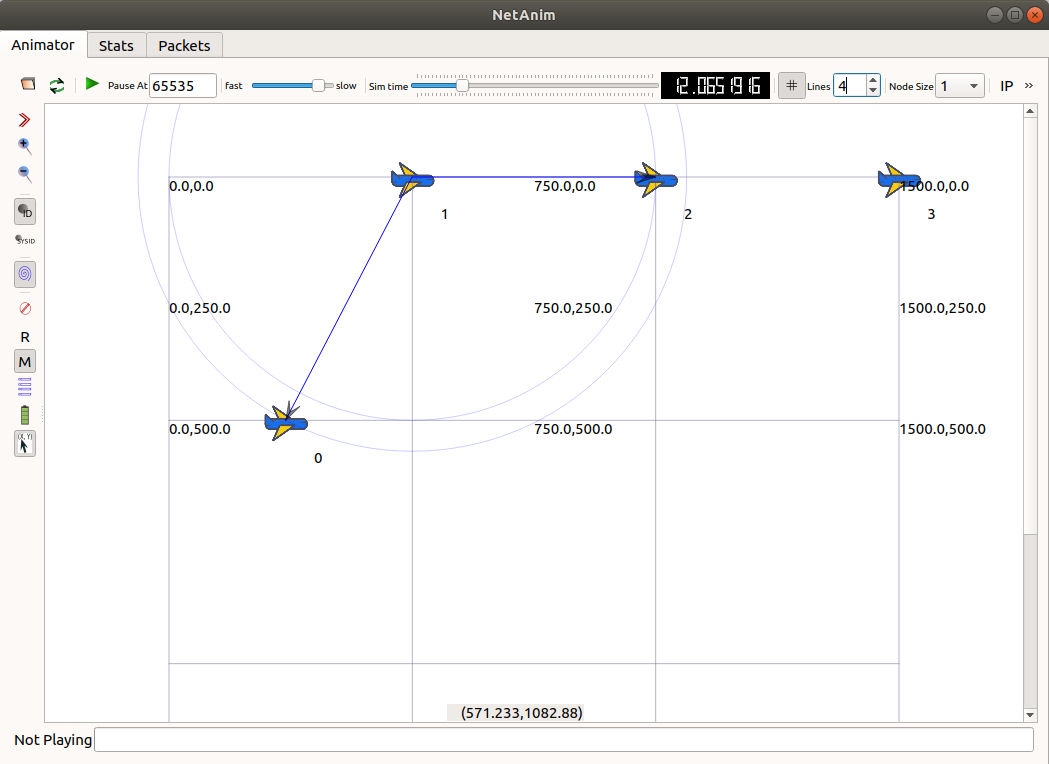
\includegraphics [width=0.6\textwidth]{figure//topo.png}
	\caption{仿真实验拓扑}\label{topo}
\end{figure}

\section{数据分析}
为了便于比较hello报文和tc报文对路由收敛的影响,本实验分别采集了hello报文和tc四组不同的设置值时路由表的收敛变化情况,具体如图1.2所示
,在图中子图(a)是hello报文设置为2s,tc报文设置为5s时的数据采集图,子图(b)(c)(d)对应的设置为hello报文为1s、0.5s和0.2s,对应的tc报
文为2.5s、1s和0.4s。

\begin{figure}[hbtp]
\centering
\begin{subfigure}[t]{0.4\textwidth}
\centering
	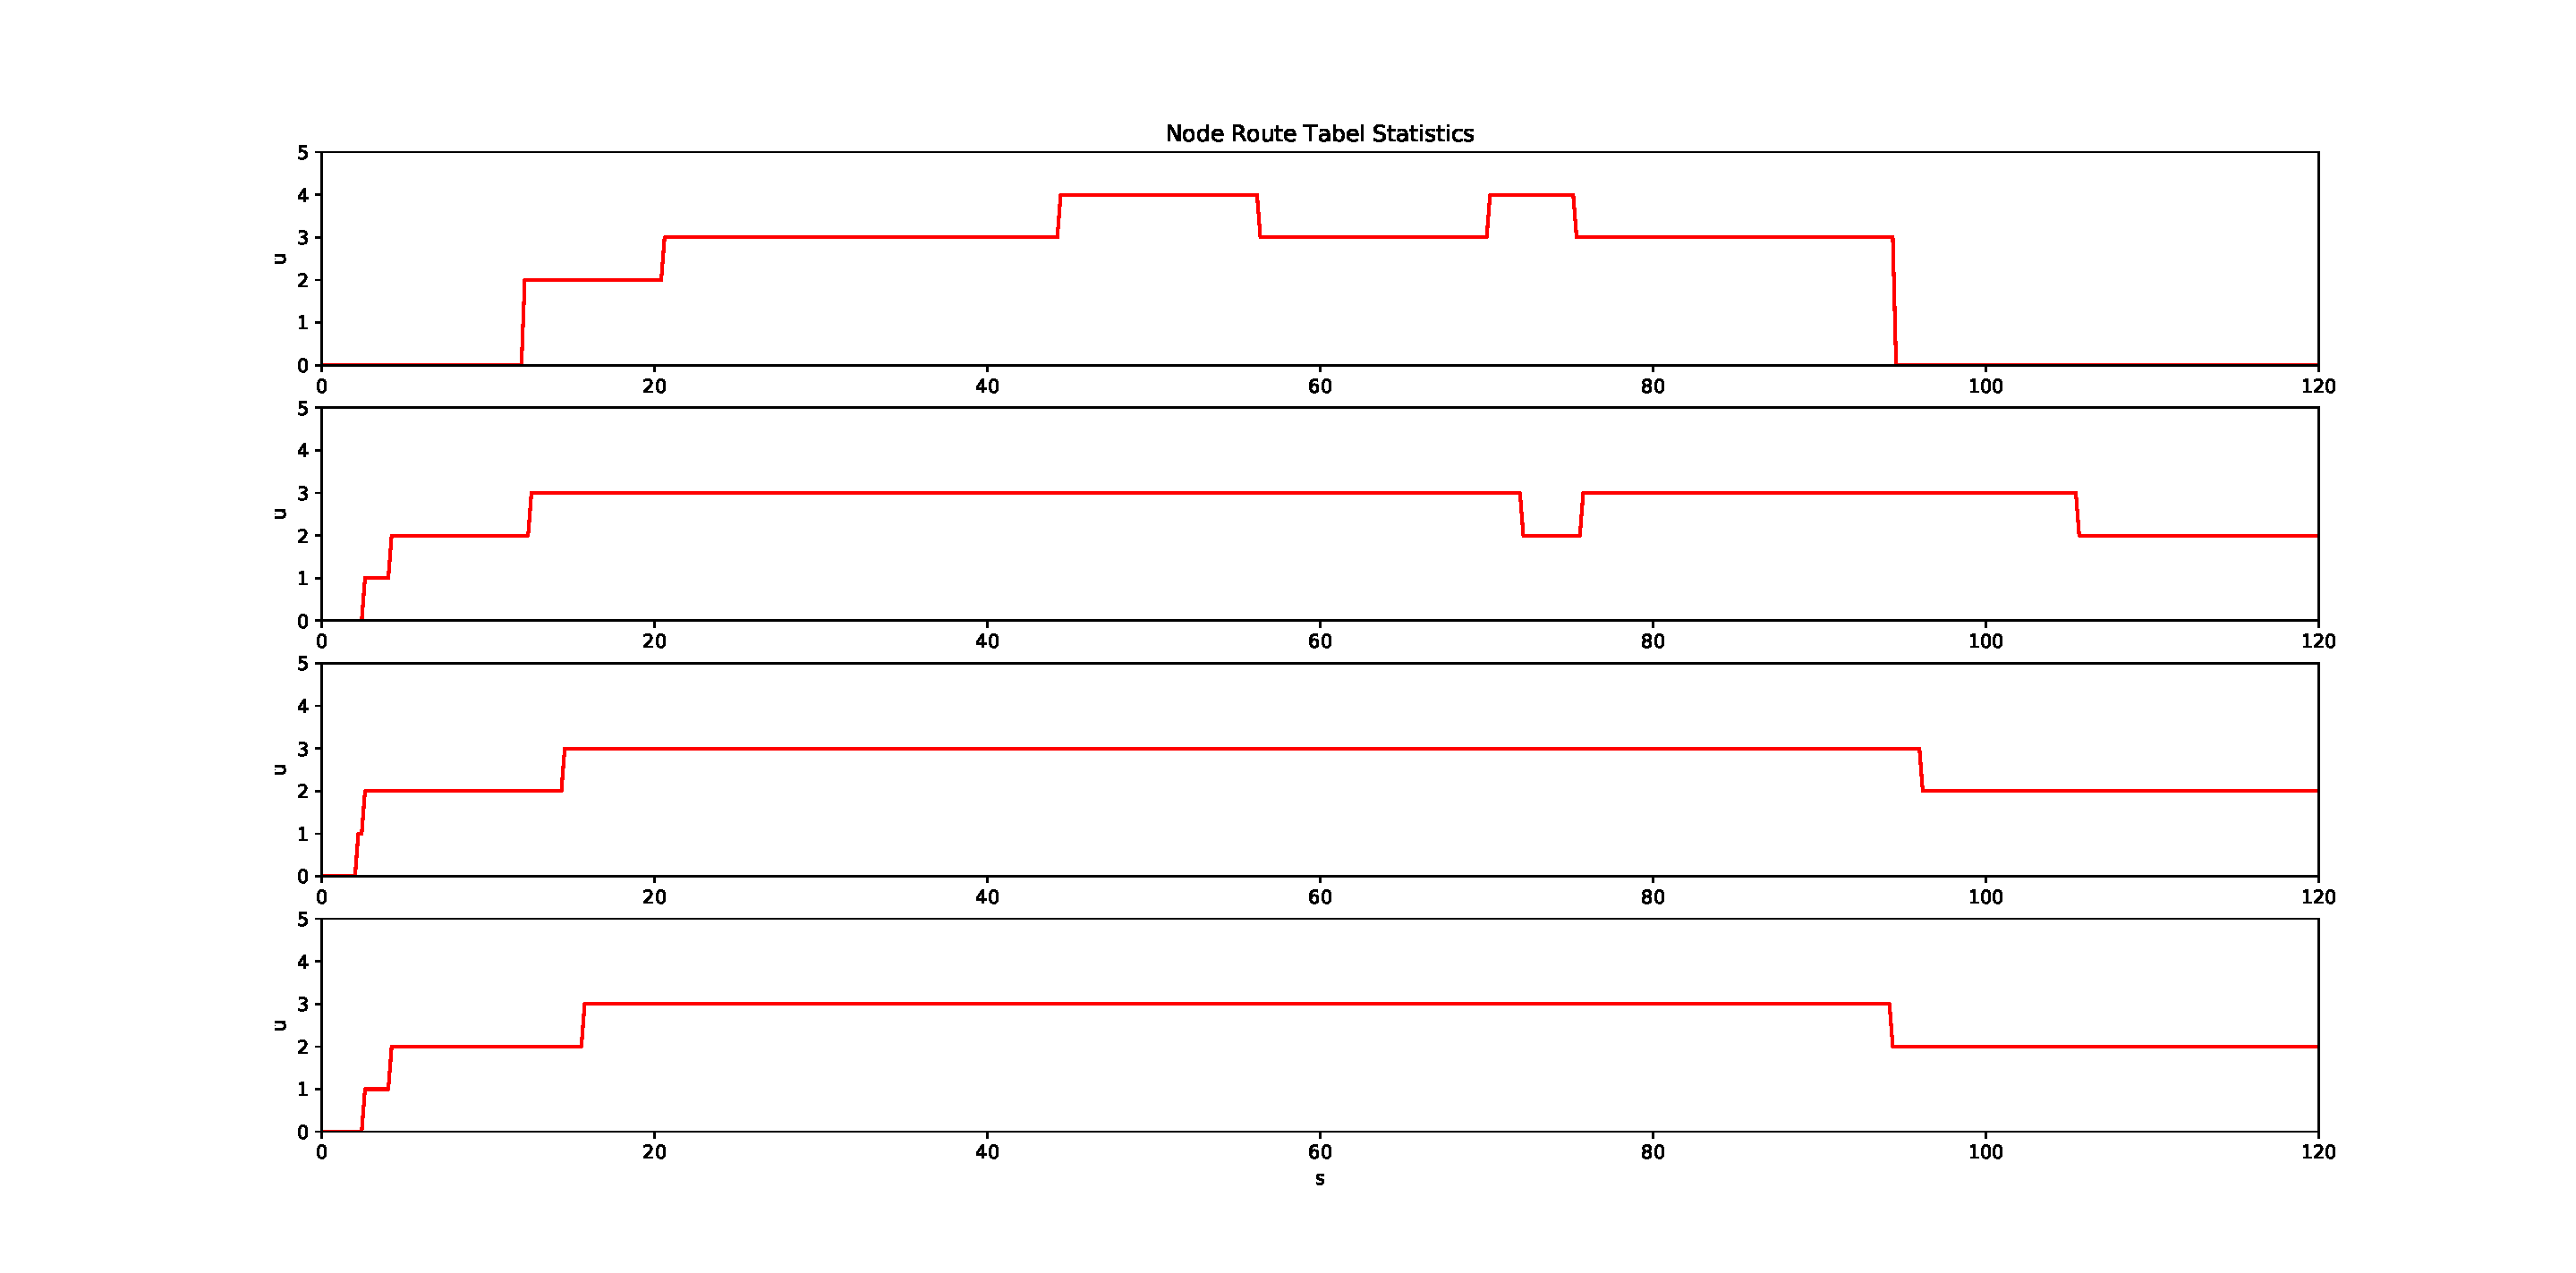
\includegraphics [width=1\textwidth]{figure//route1.pdf}
	\subcaption{hello 2s}
\end{subfigure}
\quad
\begin{subfigure}[t]{0.4\textwidth}
\centering
	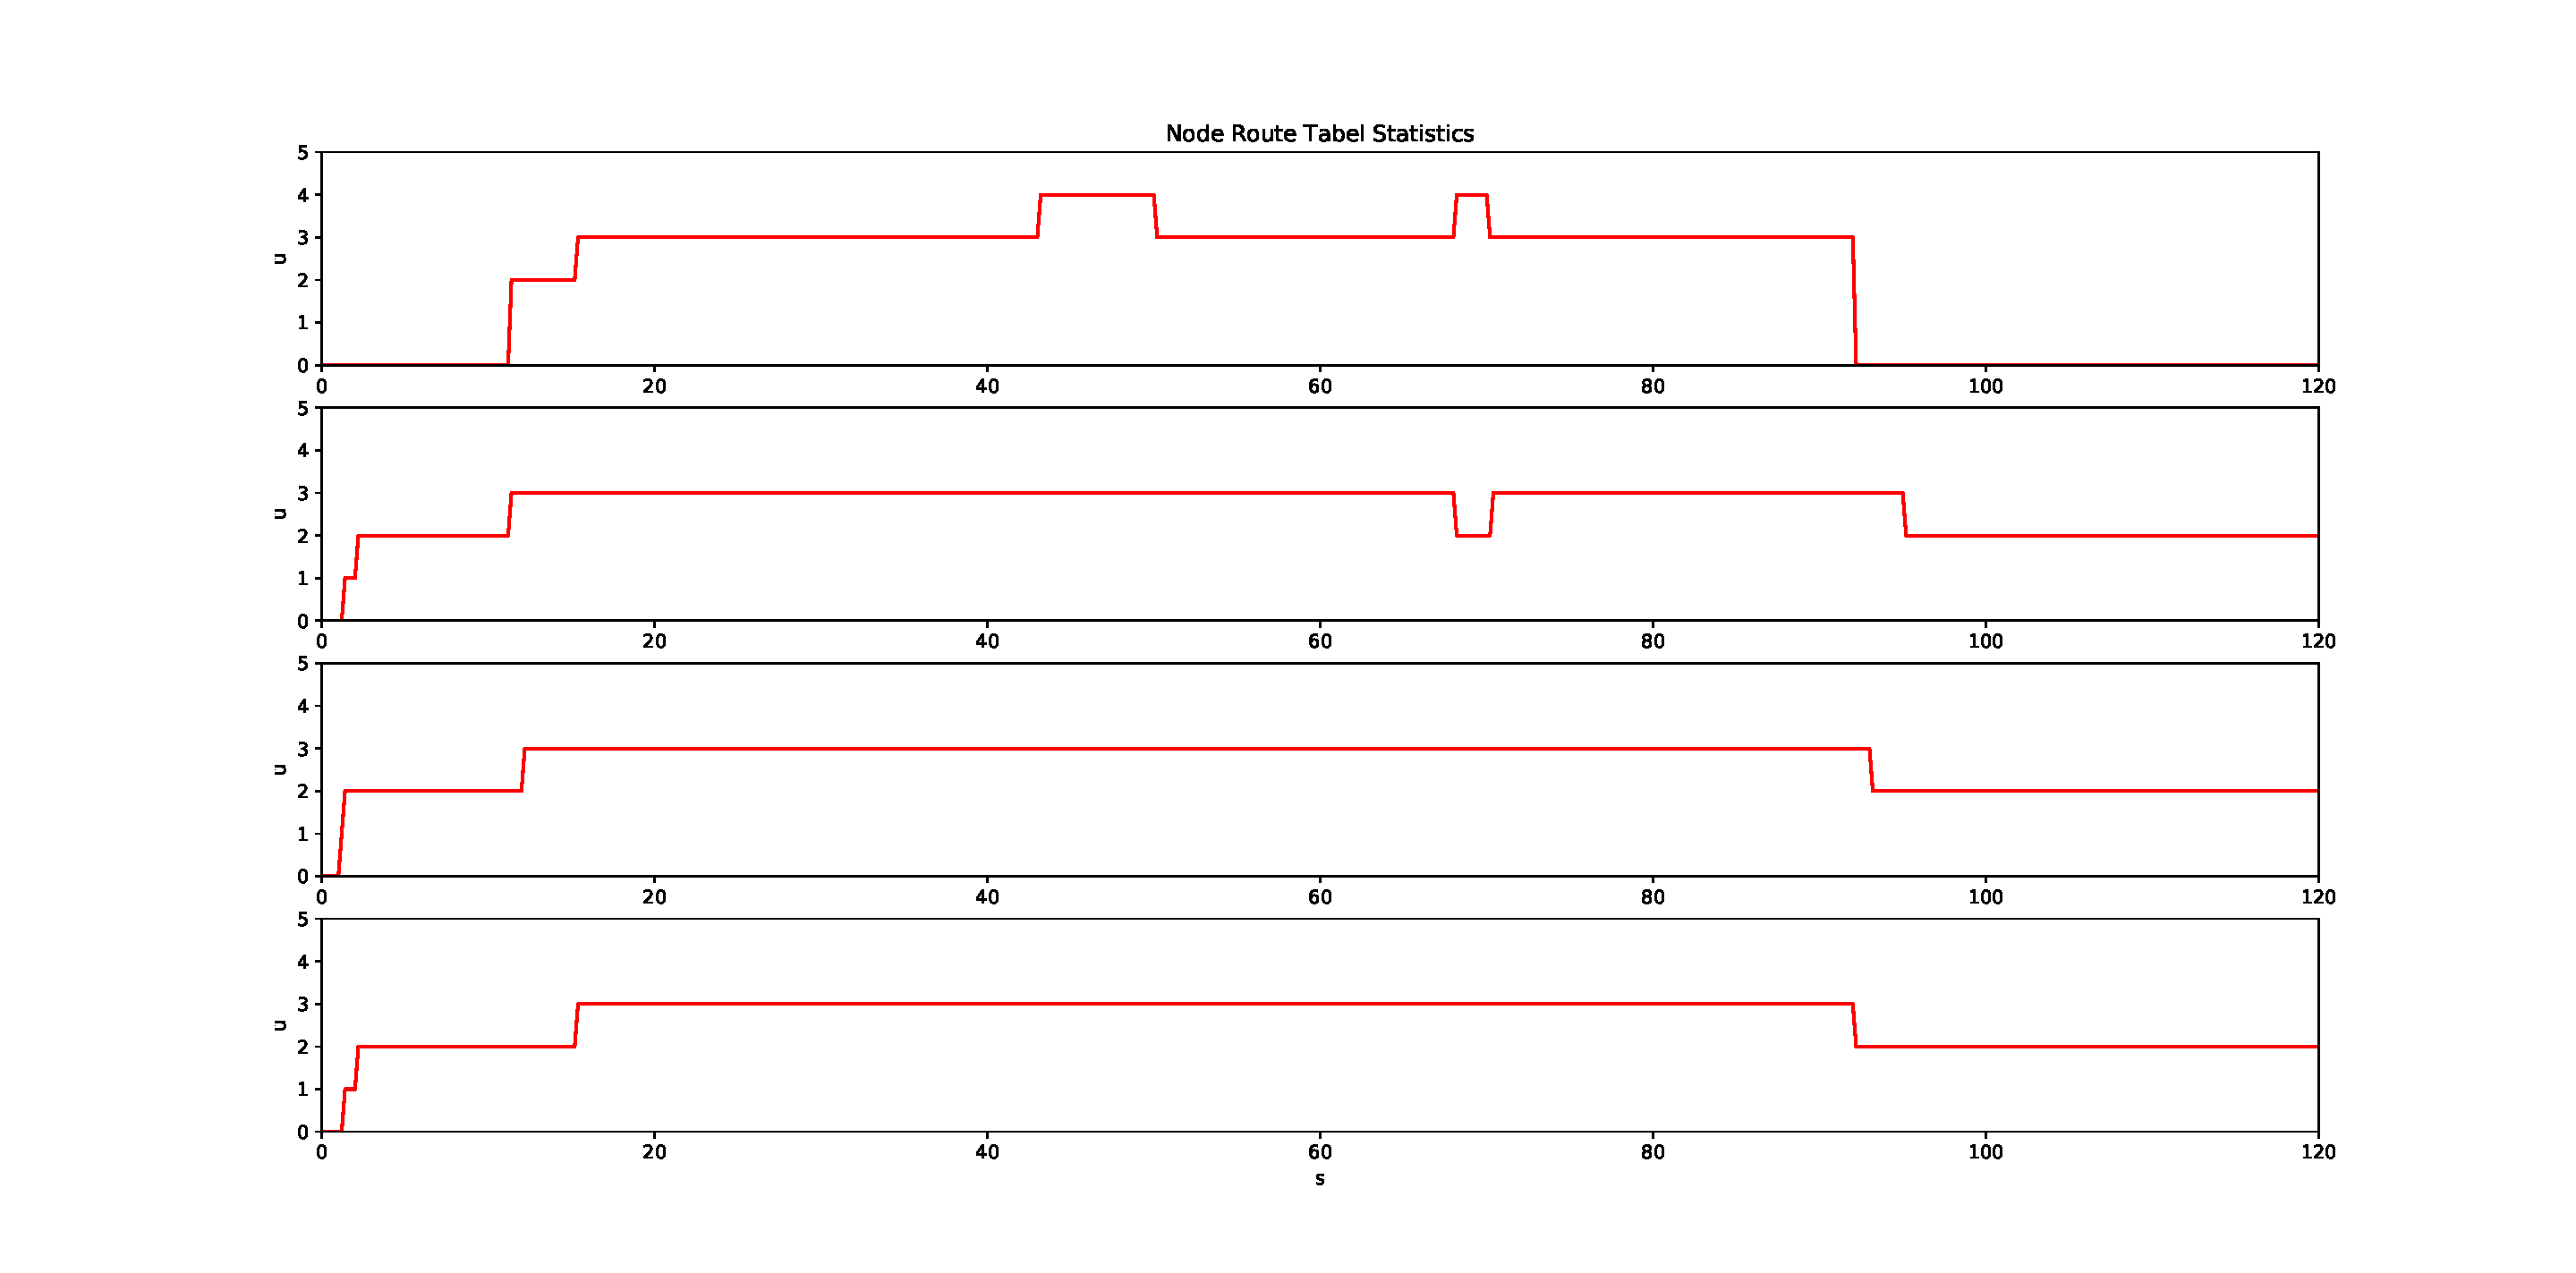
\includegraphics [width=1\textwidth]{figure//route2.pdf}
	\subcaption{hello 1s}
\end{subfigure}

\begin{subfigure}[t]{0.4\textwidth}
\centering
	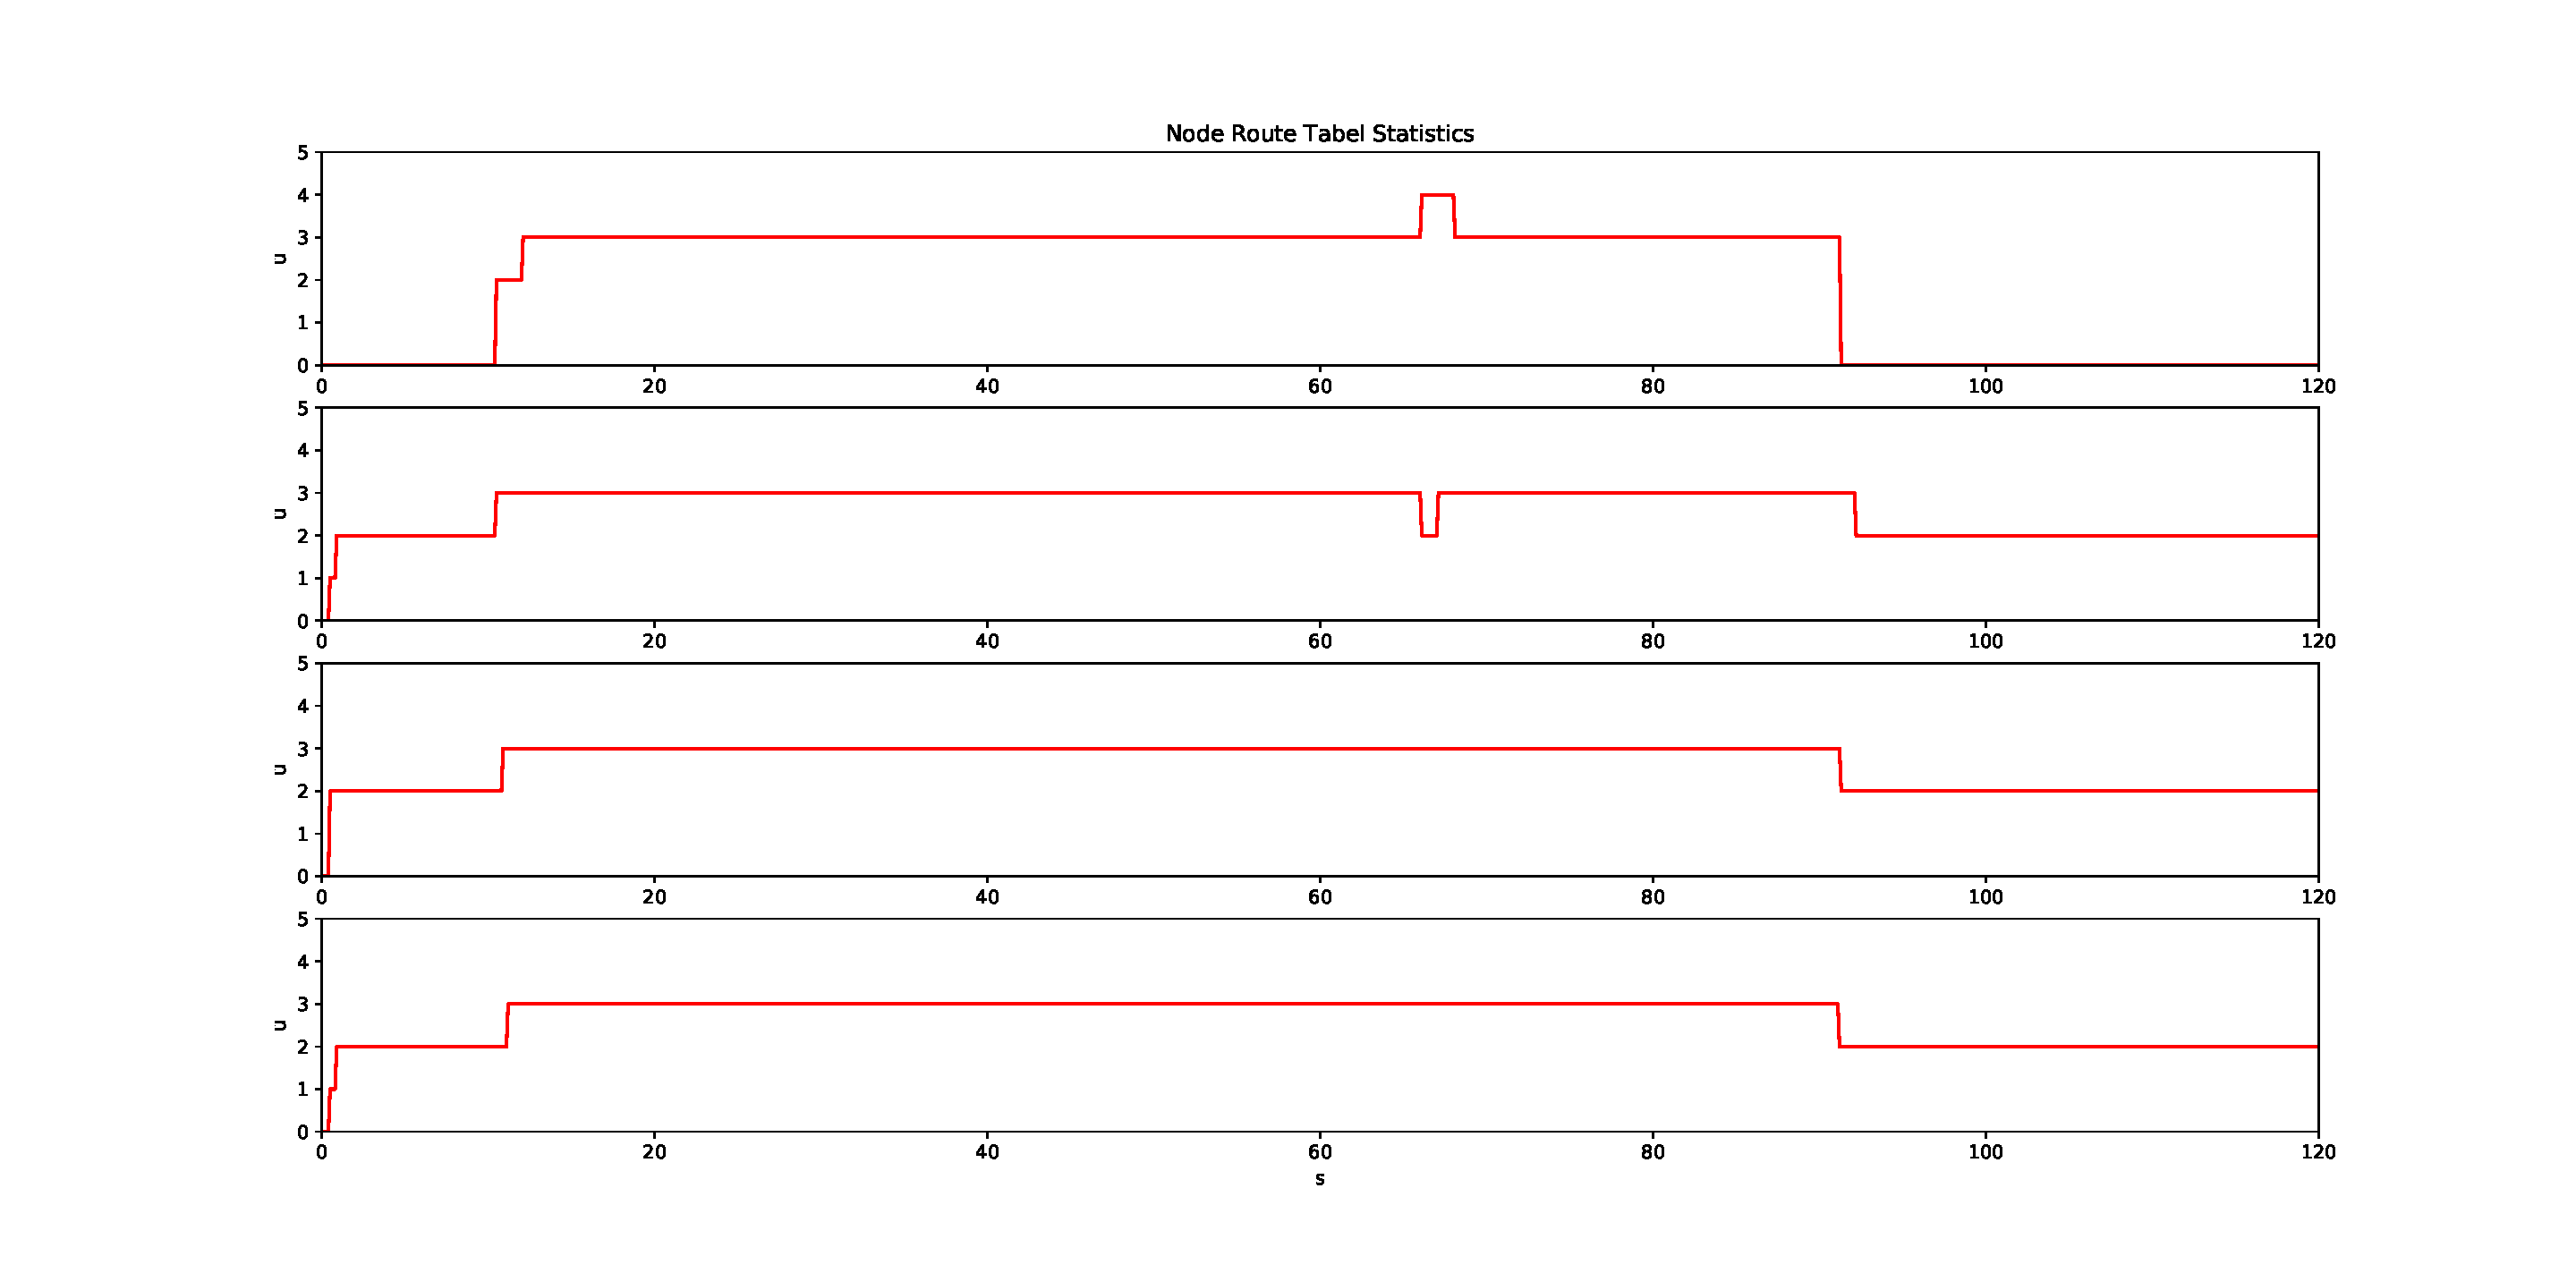
\includegraphics [width=1\textwidth]{figure//route3.pdf}
	\subcaption{hello 0.4s}
\end{subfigure}
\quad
\begin{subfigure}[t]{0.4\textwidth}
\centering
	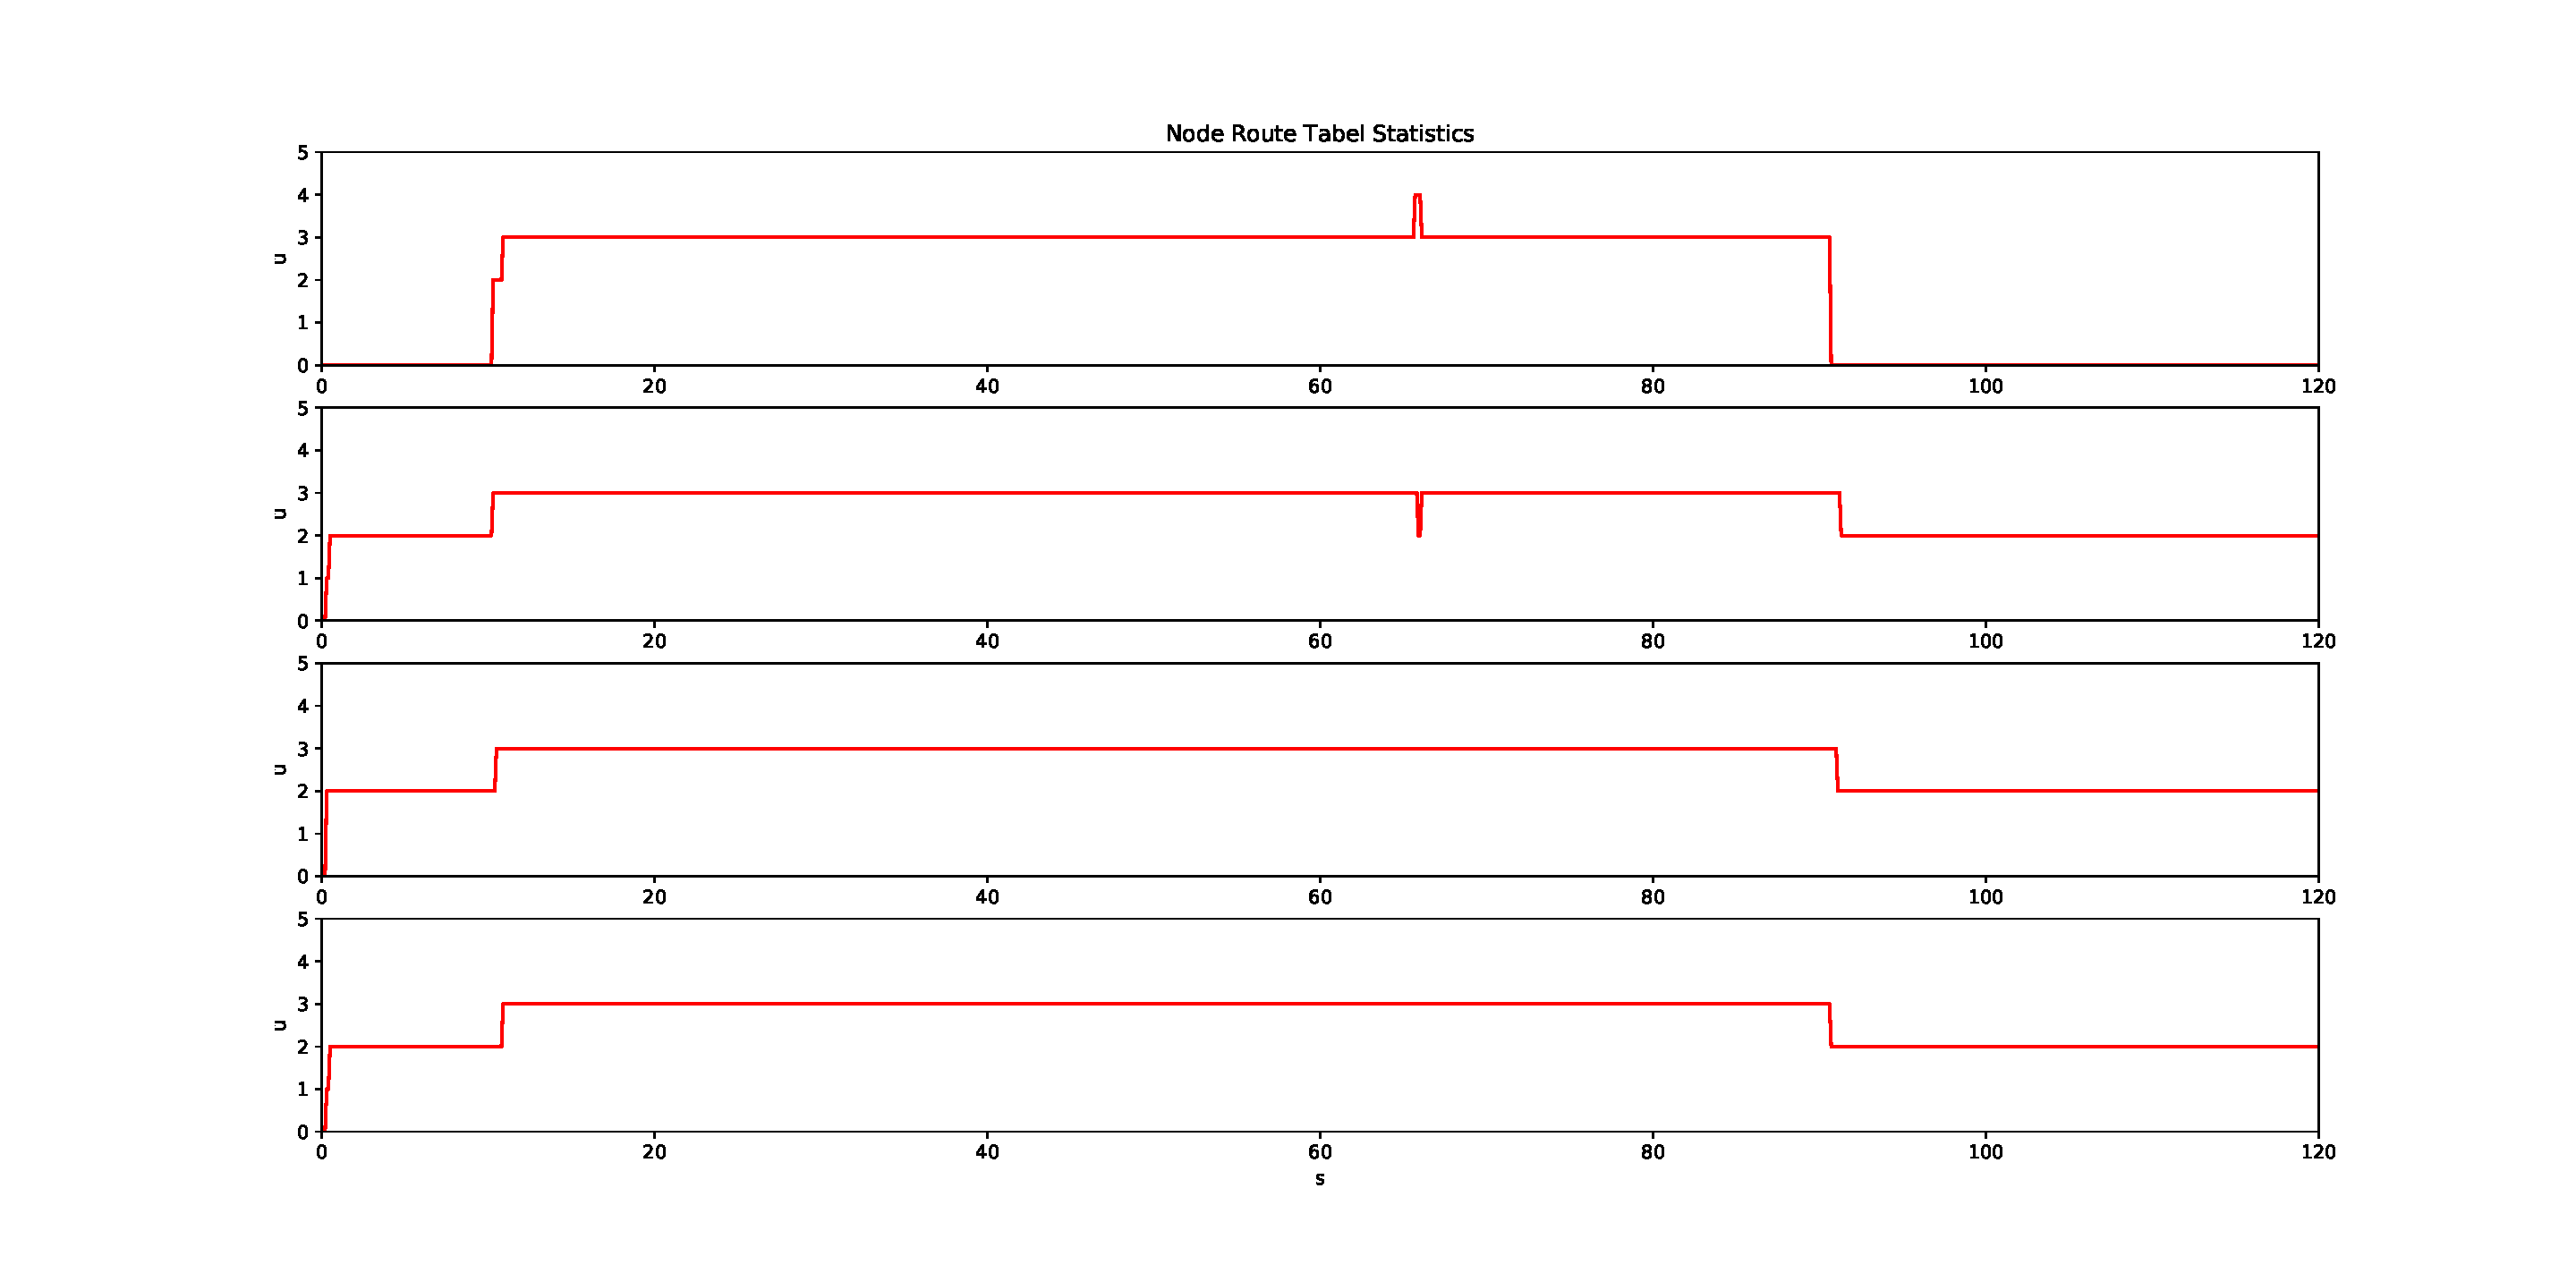
\includegraphics [width=1\textwidth]{figure//route4.pdf}
	\subcaption{hello 0.2s}
\end{subfigure}
\caption{路由数据统计}\label{figure1}
\end{figure}


根据子图(a)中仿真采集的路由表数据,可以很直接看到图中依次是node0到node3四个节点的路由表条目统计,又图中的路由项的变化可以很直
观的看到路由逐条增加,即节点之间开始组网,最开始是1号、2号、3号节点相互组网,时间基本是一致的,都是在2.6s左右的时间开始形成路由,但
是图中还是有路由异常变动的地方,对应的异常变动点后面会依次进行分析。

\begin{figure}[hbtp]
	\centering
	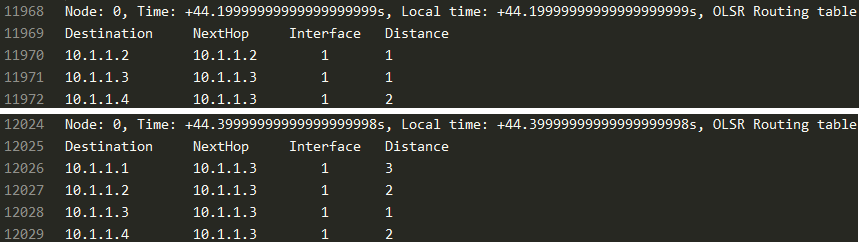
\includegraphics [width=0.8\textwidth]{figure//0-1.png}
	\caption{节点0异常变动点}\label{node0}
\end{figure}


可以先来分析一下节点0出现的异常情况,针对异常变动点的时间找到了原文件中的路由变化如图1.3所示,在路由记录文件中可以看到节点0居然多出了
一条路由,这条路由是节点0自己的路由,这应该是出现bug或者记录出错了,形成了环回路由,这应该是错误的。

\begin{figure}[hbtp]
	\centering
	\begin{subfigure}[t]{0.8\textwidth}
	\centering
	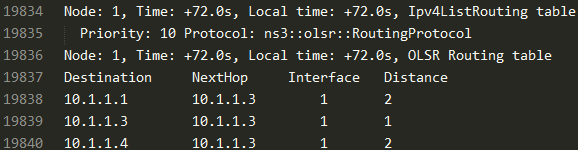
\includegraphics [width=1\textwidth]{figure//1-1.png}
	\end{subfigure}
	\begin{subfigure}[t]{0.8\textwidth}
	\centering
	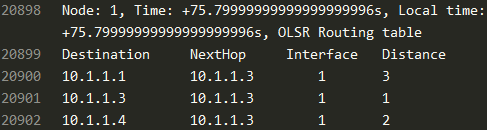
\includegraphics [width=1\textwidth]{figure//1-2.png}
	\end{subfigure}
	\caption{节点1路由变化}\label{node1}
\end{figure}


针对(a)子图异常点找到了对应的找到了节点1此时的路由,对比如图1.4所示。个点的路由变化从截图很容易看出来,1号点从与0好点直连切换到了与
0号点的通信需要2号点做中继,但是这个路由切换非常迅速,在实验中采用的是0.2s打印一次路由表,对比结果可以看出来,在0.2s内路由便实现了切
换,这个切换时间是很快的,已经达到了毫秒级。

\begin{figure}[hbtp]
	\centering
	\begin{subfigure}[t]{0.8\textwidth}
	\centering
	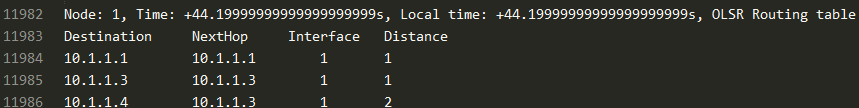
\includegraphics [width=1\textwidth]{figure//2-1.png}
	\end{subfigure}
	\begin{subfigure}[t]{0.8\textwidth}
	\centering
	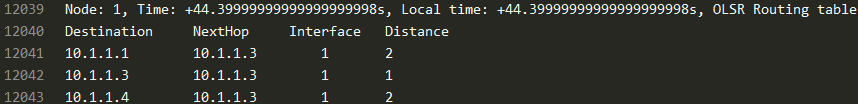
\includegraphics [width=1\textwidth]{figure//2-2.png}
	\end{subfigure}
	\caption{节点1路由变化}\label{node2}
\end{figure}

在另外的一个路由切换点则路由切换时间要长的多,根据图1.5可以得到,路由切换时间达到了3.7s。同时可以对比(b)(c)(d)图,随着hello报文和
tc报文间隔的缩小,路由切换时间也在变短。


根据节点运行轨迹,对应画了一下拓扑的变化情况,如图1.5所示,节点拓扑变化非常简单,做了两次路由切换,这期间发生了两次的路由切换,第一次
切换时间非常短,但是第二次路由切换的时候则出现了长时间路由未收敛的情况,根据参考OLSR协议的RFC文档\cite{rfc3626.olsr},在此处应该出现了MPRs的重新选举,
从而导致对整个拓扑路由的重新计算。
\begin{figure}[hbtp]
\centering
\begin{tikzpicture}
    \Vertex[x=0, y=-1.6]{A}
    \Vertex[x=0]{B} \Vertex[x=1.6]{C} \Vertex[x=3.2]{D}
    \Edge(A)(B) \Edge(B)(C) \Edge(C)(D)
    \Vertex[x=6.4]{E} \Vertex[x=8]{F} \Vertex[x=9.6]{G}
    \Vertex[x=8, y=-1.6]{H}
    \Edge(E)(F) \Edge(F)(G) \Edge(F)(H)
    \draw[line width=3pt, -latex](4, -0.8) -- (5.6, -0.8);

	\Vertex[x=1.6, y=-4.8]{A}
    \Vertex[x=0, y=-3.2]{B} \Vertex[x=1.6, y=-3.2]{C} \Vertex[x=3.2,y=-3.2]{D}
    \Edge(A)(C) \Edge(B)(C) \Edge(C)(D)
    \Vertex[x=6.4, y=-3.2]{E} \Vertex[x=8,y=-3.2]{F} \Vertex[x=9.6,y=-3.2]{G}
    \Vertex[x=9.6, y=-4.8]{H}
    \Edge(E)(F) \Edge(F)(G) \Edge(G)(H)
    \draw[line width=3pt, -latex](4, -4) -- (5.6, -4);
\end{tikzpicture}
\caption{拓扑变化图}
\end{figure}


\section{实验结论}
本实验的结论:协议路由切换时间与hello报文和tc报文正相关,hello报文和tc报文设置的越小,路由表更新时间越快。

\end{spacing}

%---------------------------------------------------------------------
%  实验二
%---------------------------------------------------------------------
\chapter{路由切换与数据传输}

\begin{spacing}{1.5}
\section{实验目的}
本实验的目的是验证olsr协议报文时钟与网络中报文数据量之间的关系。
\section{实验工具}
同上一实验。
\section{实验设计}
实验拓扑仍然采用图1.1所示,通过设置不同的hello和tc报文时钟,然后计算整个拓扑中OLSR协议的报文流通量再除以整个测试时间计算式如下:

\begin{proposition}[OLSR协议流量计算]
	数学表达式:
	\[(\sum_{i=1}^n X_i)/t \overset{\textnormal{p.s.}}{\longrightarrow} \mathbb{E} (X_i) .\]
	其中X$i$表示i节点发出的报文总数,t表示拓扑测试时间。
\end{proposition}

根据公式,分别设置了四组hello和tc报文时钟,分别是(2.0, 5.0),(1.0, 2.5), (0.5, 1), (0.2, 0.4),然后运行过程中使用wireshark统计
了各个节点的数据流量,记录了拓扑测试时间。


\section{数据分析}
在图2.1中记录了四组时钟情况下的流通量,根据图可以看到,随着hello报文和tc报文时钟的变短,报文量快速上升,基本上呈现一个线性上升的关
系,而且上升趋势比较平缓,处于可以接受的范围内。
\begin{figure}[hbtp]
\centering
\begin{tikzpicture}
	\draw [ycomb, color = blue!20, line width = 0.5 cm]
	plot coordinates{(1.5,0.557) (3,1.101) (4.5,2.735) (6,5.217)};
	\coordinate [label=above:{$5.57$}](A) at (1.5,0.6);
	\coordinate [label=above:{$11.01$}](A) at (3,1.2);
	\coordinate [label=above:{$27.35$}](A) at (4.5,3);
	\coordinate [label=above:{$52.19$}](A) at (6,5.5);
	\draw (1.5, -0.1) node [below] {2.0/5.0} -- (1.5, 0.1)
	(3, -0.1) node [below] {1.0/2.5} -- (3, 0.1)
	(4.5, -0.1) node [below] {0.4/1.0} -- (4.5, 0.1)
	(6, -0.1) node [below] {0.2/0.4} -- (6, 0.1);
	%\foreach \i in {1,2,3,4}
	%\draw (-0.1, \i) node [left] {\i} -- (0.1, \i);
	\draw (-0.1, 1) node [left] {10} -- (0.1, 1)
	(-0.1, 2) node [left] {20} -- (0.1, 2)
	(-0.1, 3) node [left] {30} -- (0.1, 3)
	(-0.1, 4) node [left] {40} -- (0.1, 4)
	(-0.1, 5) node [left] {50} -- (0.1, 5)
	(-0.1, 6) node [left] {60} -- (0.1, 6);

	\draw [<->] (0,6.5) node [above] {$kbps$}
	-- (0,0)
	-- (6.5,0) node [right] {$hello/tc$} ;
\end{tikzpicture}
\caption{报文数据流量}
\end{figure}


同时我们关心单位时间内报文流量的情况在当hello和tc报文分别设置到(0.2, 0.4),根据图1.2的(d)子图可以看到,路由切换基本能够满足在
300ms左右完成切换,且此时流量维持在52kbps左右,这样的流量大小和切换时延是能够接受的。

\section{实验结论}
本实验结论:一定程度上缩短hello报文和tc报文的时钟,可以加速路由表的切换,且拓扑中所增加的报文流量是能够接受和可以预期的。
\end{spacing}

%---------------------------------------------------------------------
%  实验感想
%---------------------------------------------------------------------
\titleformat{\chapter}{\centering\zihao{-1}\heiti}{}{1em}{}
\chapter{实验总结}
\begin{spacing}{1.5}
通过本次仿真实验加深了对于OLSR协议的理解,也从理论上指导了在设备上调试运行OLSR协议,并且为后续针对OLSR协议的改进打下了良好的基
础。
\end{spacing}

%---------------------------------------------------------------------
%  参考文献设置
%---------------------------------------------------------------------
\addcontentsline{toc}{chapter}{参考文献}

\begin{thebibliography}{99}
\songti \zihao{-4} 	
	\bibitem{NS3.web}
	https://www.nsnam.org/
	\bibitem{rfc3626.olsr}
	Network Working Group. OLSR: Optimized Link State Routing Protocol, 2003.
	
\end{thebibliography}

%---------------------------------------------------------------------
%  附录设置
%---------------------------------------------------------------------
\titleformat{\chapter}{\heiti\Large}{附录~\Alph{chapter}}{11pt}{\Large}
\titlespacing{\chapter}{0pt}{*-4}{*4}

\lstset{breaklines}                %自动将长的代码行换行排版
\lstset{extendedchars=false}
\lstset{language=Matlab}
\renewcommand{\thechapter}{附录\Alph{chapter}.} 
\appendix
\begin{appendix}
	
	
\chapter{数据表}
\zihao{-4}\songti
\begin{spacing}{1.5}
\begin{enumerate}
\item 路由表记录文件
\item 各节点抓包文件
\end{enumerate}
\end{spacing}


\chapter{程序代码}
\zihao{-4}\songti
\begin{spacing}{1.5}
下面是ns3仿真的C++程序,分别设置了各个节点的属性和测试过程,具体可以参考代码内容。
\begin{lstlisting}[language=c++]
/* -*-  Mode: C++; c-file-style: "gnu"; indent-tabs-mode:nil; -*- */
/*
	* Copyright (c) 2009 University of Washington
	*
	* This program is free software; you can redistribute it and/or modify
	* it under the terms of the GNU General Public License version 2 as
	* published by the Free Software Foundation;
	*
	* This program is distributed in the hope that it will be useful,
	* but WITHOUT ANY WARRANTY; without even the implied warranty of
	* MERCHANTABILITY or FITNESS FOR A PARTICULAR PURPOSE.  See the
	* GNU General Public License for more details.
	*
	* You should have received a copy of the GNU General Public License
	* along with this program; if not, write to the Free Software
	* Foundation, Inc., 59 Temple Place, Suite 330, Boston, MA  02111-1307  USA
	*
	*/

//
// This program configures a grid (default 5x5) of nodes on an
// 802.11b physical layer, with
// 802.11b NICs in adhoc mode, and by default, sends one packet of 1000
// (application) bytes to node 1.
//
// The default layout is like this, on a 2-D grid.
//
// n20  n21  n22  n23  n24
// n15  n16  n17  n18  n19
// n10  n11  n12  n13  n14
// n5   n6   n7   n8   n9
// n0   n1   n2   n3   n4
//
// the layout is affected by the parameters given to GridPositionAllocator;
// by default, GridWidth is 5 and numNodes is 25..
//
// There are a number of command-line options available to control
// the default behavior.  The list of available command-line options
// can be listed with the following command:
// ./waf --run "wifi-simple-adhoc-grid --help"
//
// Note that all ns-3 attributes (not just the ones exposed in the below
// script) can be changed at command line; see the ns-3 documentation.
//
// For instance, for this configuration, the physical layer will
// stop successfully receiving packets when distance increases beyond
// the default of 500m.
// To see this effect, try running:
//
// ./waf --run "wifi-simple-adhoc --distance=500"
// ./waf --run "wifi-simple-adhoc --distance=1000"
// ./waf --run "wifi-simple-adhoc --distance=1500"
//
// The source node and sink node can be changed like this:
//
// ./waf --run "wifi-simple-adhoc --sourceNode=20 --sinkNode=10"
//
// This script can also be helpful to put the Wifi layer into verbose
// logging mode; this command will turn on all wifi logging:
//
// ./waf --run "wifi-simple-adhoc-grid --verbose=1"
//
// By default, trace file writing is off-- to enable it, try:
// ./waf --run "wifi-simple-adhoc-grid --tracing=1"
//
// When you are done tracing, you will notice many pcap trace files
// in your directory.  If you have tcpdump installed, you can try this:
//
// tcpdump -r wifi-simple-adhoc-grid-0-0.pcap -nn -tt
//

#include "ns3/core-module.h"
#include "ns3/mobility-module.h"
#include "ns3/wifi-module.h"
#include "ns3/internet-module.h"
#include "ns3/olsr-helper.h"

#include "ns3/netanim-module.h"

using namespace ns3;

NS_LOG_COMPONENT_DEFINE ("WifiSimpleAdhocGrid");

void ReceivePacket (Ptr<Socket> socket)
{
	while (socket->Recv ())
	{
		NS_LOG_UNCOND ("Received one packet!");
	}
}

static void GenerateTraffic (Ptr<Socket> socket, uint32_t pktSize,
								uint32_t pktCount, Time pktInterval )
{
	if (pktCount > 0)
	{
		socket->Send (Create<Packet> (pktSize));
		Simulator::Schedule (pktInterval, &GenerateTraffic,
							socket, pktSize,pktCount - 1, pktInterval);
	}
	else
	{
		socket->Close ();
	}
}


int main (int argc, char *argv[])
{
	std::string phyMode ("DsssRate1Mbps");
	double distance = 500;  // m
	uint32_t packetSize = 1000; // bytes
	uint32_t numPackets = 100;
	uint32_t numNodes = 4;  // by default, 5x5
	uint32_t sinkNode = 0;
	uint32_t sourceNode = 3;
	double interval = 1.0; // seconds
	bool verbose = false;
	bool tracing = false;
	double HelloInterval = 2.0;
	double TcInterval = 5.0;
	double MidInterval = 5.0;
	double HnaInterval = 5.0;

	CommandLine cmd;

	cmd.AddValue ("phyMode", "Wifi Phy mode", phyMode);
	cmd.AddValue ("distance", "distance (m)", distance);
	cmd.AddValue ("packetSize", "size of application packet sent", packetSize);
	cmd.AddValue ("numPackets", "number of packets generated", numPackets);
	cmd.AddValue ("interval", "interval (seconds) between packets", interval);
	cmd.AddValue ("verbose", "turn on all WifiNetDevice log components", verbose);
	cmd.AddValue ("tracing", "turn on ascii and pcap tracing", tracing);
	cmd.AddValue ("numNodes", "number of nodes", numNodes);
	cmd.AddValue ("sinkNode", "Receiver node number", sinkNode);
	cmd.AddValue ("sourceNode", "Sender node number", sourceNode);
	cmd.AddValue ("hellointerval", "OLSR Routing Protocol hello packet interval", HelloInterval);
	cmd.AddValue ("tcinterval", "OLSR Routing Protocol Tc packet interval", TcInterval);
	cmd.AddValue ("midinterval", "OLSR Routing Protocol Mid interval", MidInterval);
	cmd.AddValue ("hnainterval", "OLSR Routing Protocol Hna interval", HnaInterval);

	cmd.Parse (argc, argv);
	// Convert to time object
	Time interPacketInterval = Seconds (interval);

	// disable fragmentation for frames below 2200 bytes
	Config::SetDefault ("ns3::WifiRemoteStationManager::FragmentationThreshold", StringValue ("2200"));
	// turn off RTS/CTS for frames below 2200 bytes
	Config::SetDefault ("ns3::WifiRemoteStationManager::RtsCtsThreshold", StringValue ("2200"));
	// Fix non-unicast data rate to be the same as that of unicast
	Config::SetDefault ("ns3::WifiRemoteStationManager::NonUnicastMode",
						StringValue (phyMode));

	NodeContainer c;
	c.Create (numNodes);

	// The below set of helpers will help us to put together the wifi NICs we want
	WifiHelper wifi;
	if (verbose)
	{
		wifi.EnableLogComponents ();  // Turn on all Wifi logging
	}

	YansWifiPhyHelper wifiPhy =  YansWifiPhyHelper::Default ();
	// set it to zero; otherwise, gain will be added
	wifiPhy.Set ("RxGain", DoubleValue (-10) );
	// ns-3 supports RadioTap and Prism tracing extensions for 802.11b
	wifiPhy.SetPcapDataLinkType (WifiPhyHelper::DLT_IEEE802_11_RADIO);

	YansWifiChannelHelper wifiChannel;
	wifiChannel.SetPropagationDelay ("ns3::ConstantSpeedPropagationDelayModel");
	wifiChannel.AddPropagationLoss ("ns3::FriisPropagationLossModel");
	wifiPhy.SetChannel (wifiChannel.Create ());

	// Add an upper mac and disable rate control
	WifiMacHelper wifiMac;
	wifi.SetStandard (WIFI_PHY_STANDARD_80211b);
	wifi.SetRemoteStationManager ("ns3::ConstantRateWifiManager",
								"DataMode",StringValue (phyMode),
								"ControlMode",StringValue (phyMode));
	// Set it to adhoc mode
	wifiMac.SetType ("ns3::AdhocWifiMac");
	NetDeviceContainer devices = wifi.Install (wifiPhy, wifiMac, c);

	MobilityHelper mobility;
	mobility.SetPositionAllocator ("ns3::GridPositionAllocator",
									"MinX", DoubleValue (0.0),
									"MinY", DoubleValue (0.0),
									"DeltaX", DoubleValue (distance),
									"DeltaY", DoubleValue (distance),
									"GridWidth", UintegerValue (4),
									"LayoutType", StringValue ("RowFirst"));
	//mobility.SetMobilityModel ("ns3::ConstantPositionMobilityModel");
	mobility.SetMobilityModel ("ns3::ConstantVelocityMobilityModel");
	mobility.Install (c);

	c.Get (0)->GetObject<MobilityModel> ()->SetPosition (Vector (0, 500, 0));
	c.Get (0)->GetObject<ConstantVelocityMobilityModel> ()->SetVelocity (Vector (20, 0, 0));

	// Enable OLSR
	OlsrHelper olsr;
	Ipv4StaticRoutingHelper staticRouting;

	Time t_HelloInterval = Seconds (HelloInterval);
	olsr.Set("HelloInterval", TimeValue(t_HelloInterval));

	Time t_TcInterval = Seconds (TcInterval);
	olsr.Set("TcInterval", TimeValue(t_TcInterval));

	Time t_MidInterval = Seconds (MidInterval);
	olsr.Set("MidInterval", TimeValue(t_MidInterval));

	Time t_HnaInterval = Seconds (HnaInterval);
	olsr.Set("HnaInterval", TimeValue(t_HnaInterval));


	Ipv4ListRoutingHelper list;
	list.Add (staticRouting, 0);
	list.Add (olsr, 10);

	InternetStackHelper internet;
	internet.SetRoutingHelper (list); // has effect on the next Install ()
	internet.Install (c);

	Ipv4AddressHelper ipv4;
	NS_LOG_INFO ("Assign IP Addresses.");
	ipv4.SetBase ("10.1.1.0", "255.255.255.0");
	Ipv4InterfaceContainer i = ipv4.Assign (devices);

	TypeId tid = TypeId::LookupByName ("ns3::UdpSocketFactory");
	Ptr<Socket> recvSink = Socket::CreateSocket (c.Get (sinkNode), tid);
	InetSocketAddress local = InetSocketAddress (Ipv4Address::GetAny (), 80);
	recvSink->Bind (local);
	recvSink->SetRecvCallback (MakeCallback (&ReceivePacket));

	Ptr<Socket> source = Socket::CreateSocket (c.Get (sourceNode), tid);
	InetSocketAddress remote = InetSocketAddress (i.GetAddress (sinkNode, 0), 80);
	source->Connect (remote);

	if (tracing == true)
	{
		AsciiTraceHelper ascii;
		wifiPhy.EnableAsciiAll (ascii.CreateFileStream ("wifi-simple-adhoc-grid.tr"));
		wifiPhy.EnablePcap ("wifi-simple-adhoc-grid", devices);
		// Trace routing tables
		Ptr<OutputStreamWrapper> routingStream = Create<OutputStreamWrapper> ("wifi-simple-adhoc-grid.routes", std::ios::out);
		olsr.PrintRoutingTableAllEvery (Seconds (0.1), routingStream);
		Ptr<OutputStreamWrapper> neighborStream = Create<OutputStreamWrapper> ("wifi-simple-adhoc-grid.neighbors", std::ios::out);
		olsr.PrintNeighborCacheAllEvery (Seconds (0.1), neighborStream);

		// To do-- enable an IP-level trace that shows forwarding events only
	}

	// Give OLSR time to converge-- 30 seconds perhaps
	Simulator::Schedule (Seconds (120.0), &GenerateTraffic,
						source, packetSize, numPackets, interPacketInterval);

	// Output what we are doing
	NS_LOG_UNCOND ("Testing from node " << sourceNode << " to " << sinkNode << " with grid distance " << distance);

	Simulator::Stop (Seconds (123.0));

	AnimationInterface anim("olsr-adhoc.xml");

	Simulator::Run ();
	Simulator::Destroy ();

	return 0;
}
\end{lstlisting}
\end{spacing}
\end{appendix}
		

\end{document}